\documentclass[tikz,border=5pt]{standalone}
\usepackage{amsmath,amssymb,txfonts}
\usetikzlibrary{arrows.meta,positioning,fit,calc}
\newcommand{\gcode}{G_{\mathrm{code}}}
\newcommand{\gstate}{G_{\mathrm{state}}}
\begin{document}
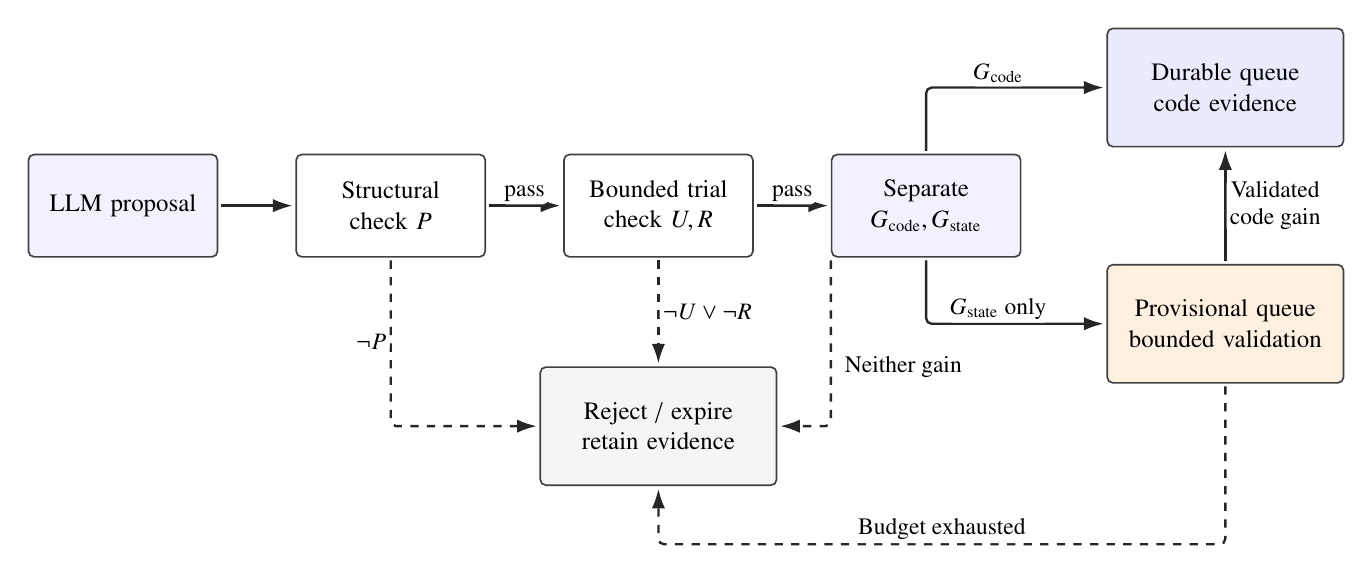
\begin{tikzpicture}[
  font=\fontsize{9}{11}\selectfont,
  box/.style={draw=black!75,line width=0.6pt,rounded corners=2pt,
    align=center,text width=21mm,minimum width=24mm,
    minimum height=13mm,inner sep=3pt},
  queue/.style={box,text width=27mm,minimum width=30mm,
    minimum height=15mm},
  flow/.style={-{Latex[length=2.5mm,width=1.7mm]},
    draw=black!85,line width=0.85pt,rounded corners=2pt,
    shorten <=1pt,shorten >=1pt},
  failure/.style={flow,dashed},
  condition/.style={font=\fontsize{8.5}{10}\selectfont,
    text=black,fill=white,inner sep=1.2pt,align=center}]
\node[box,fill=blue!5] (llm) at (0,0) {LLM proposal};
\node[box] (p) at (3.4,0) {Structural\\check $P$};
\node[box] (trial) at (6.8,0) {Bounded trial\\check $U,R$};
\node[box,fill=blue!5] (gain) at (10.2,0) {Separate\\$\gcode,\gstate$};
\node[queue,fill=blue!8] (dur) at (14,1.5) {Durable queue\\code evidence};
\node[queue,fill=orange!12] (prov) at (14,-1.5) {Provisional queue\\bounded validation};
\node[queue,fill=black!4] (rej) at (6.8,-2.8) {Reject / expire\\retain evidence};

\draw[flow] (llm.east)--(p.west);
\draw[flow] (p.east)--node[condition,above] (p_ok) {pass}(trial.west);
\draw[flow] (trial.east)--node[condition,above] (ur_ok) {pass}(gain.west);
\draw[flow] (gain.north)|-node[condition,above,pos=.7] (code_gate) {$\gcode$}(dur.west);
\draw[flow] (gain.south)|-node[condition,above,pos=.7] (state_gate) {$\gstate$ only}(prov.west);
\draw[flow] (prov.north)--node[condition,right] (promotion) {Validated\\code gain}(dur.south);

\draw[failure] (p.south)|-node[condition,left,pos=.25] (p_fail) {$\neg P$}(rej.west);
\draw[failure] (trial.south)--node[condition,right] (ur_fail) {$\neg U\lor\neg R$}(rej.north);
\draw[failure] (gain.south west)|-(rej.east);
\node[condition,anchor=west] (no_gain) at (9.12,-2.05) {Neither gain};
\draw[failure] (prov.south)--(14,-4.3)--
  node[condition,above] (expiry) {Budget exhausted}(6.8,-4.3)--(rej.south);

\path (llm.south west);\pgfgetlastxy{\figx}{\figy}\typeout{FIG2|llm|sw|\figx|\figy}
\path (llm.north east);\pgfgetlastxy{\figx}{\figy}\typeout{FIG2|llm|ne|\figx|\figy}
\path (p.south west);\pgfgetlastxy{\figx}{\figy}\typeout{FIG2|p|sw|\figx|\figy}
\path (p.north east);\pgfgetlastxy{\figx}{\figy}\typeout{FIG2|p|ne|\figx|\figy}
\path (trial.south west);\pgfgetlastxy{\figx}{\figy}\typeout{FIG2|trial|sw|\figx|\figy}
\path (trial.north east);\pgfgetlastxy{\figx}{\figy}\typeout{FIG2|trial|ne|\figx|\figy}
\path (gain.south west);\pgfgetlastxy{\figx}{\figy}\typeout{FIG2|gain|sw|\figx|\figy}
\path (gain.north east);\pgfgetlastxy{\figx}{\figy}\typeout{FIG2|gain|ne|\figx|\figy}
\path (dur.south west);\pgfgetlastxy{\figx}{\figy}\typeout{FIG2|dur|sw|\figx|\figy}
\path (dur.north east);\pgfgetlastxy{\figx}{\figy}\typeout{FIG2|dur|ne|\figx|\figy}
\path (prov.south west);\pgfgetlastxy{\figx}{\figy}\typeout{FIG2|prov|sw|\figx|\figy}
\path (prov.north east);\pgfgetlastxy{\figx}{\figy}\typeout{FIG2|prov|ne|\figx|\figy}
\path (rej.south west);\pgfgetlastxy{\figx}{\figy}\typeout{FIG2|rej|sw|\figx|\figy}
\path (rej.north east);\pgfgetlastxy{\figx}{\figy}\typeout{FIG2|rej|ne|\figx|\figy}
\path (p_ok.south west);\pgfgetlastxy{\figx}{\figy}\typeout{FIG2|p_ok|sw|\figx|\figy}
\path (p_ok.north east);\pgfgetlastxy{\figx}{\figy}\typeout{FIG2|p_ok|ne|\figx|\figy}
\path (ur_ok.south west);\pgfgetlastxy{\figx}{\figy}\typeout{FIG2|ur_ok|sw|\figx|\figy}
\path (ur_ok.north east);\pgfgetlastxy{\figx}{\figy}\typeout{FIG2|ur_ok|ne|\figx|\figy}
\path (code_gate.south west);\pgfgetlastxy{\figx}{\figy}\typeout{FIG2|code_gate|sw|\figx|\figy}
\path (code_gate.north east);\pgfgetlastxy{\figx}{\figy}\typeout{FIG2|code_gate|ne|\figx|\figy}
\path (state_gate.south west);\pgfgetlastxy{\figx}{\figy}\typeout{FIG2|state_gate|sw|\figx|\figy}
\path (state_gate.north east);\pgfgetlastxy{\figx}{\figy}\typeout{FIG2|state_gate|ne|\figx|\figy}
\path (promotion.south west);\pgfgetlastxy{\figx}{\figy}\typeout{FIG2|promotion|sw|\figx|\figy}
\path (promotion.north east);\pgfgetlastxy{\figx}{\figy}\typeout{FIG2|promotion|ne|\figx|\figy}
\path (p_fail.south west);\pgfgetlastxy{\figx}{\figy}\typeout{FIG2|p_fail|sw|\figx|\figy}
\path (p_fail.north east);\pgfgetlastxy{\figx}{\figy}\typeout{FIG2|p_fail|ne|\figx|\figy}
\path (ur_fail.south west);\pgfgetlastxy{\figx}{\figy}\typeout{FIG2|ur_fail|sw|\figx|\figy}
\path (ur_fail.north east);\pgfgetlastxy{\figx}{\figy}\typeout{FIG2|ur_fail|ne|\figx|\figy}
\path (no_gain.south west);\pgfgetlastxy{\figx}{\figy}\typeout{FIG2|no_gain|sw|\figx|\figy}
\path (no_gain.north east);\pgfgetlastxy{\figx}{\figy}\typeout{FIG2|no_gain|ne|\figx|\figy}
\path (expiry.south west);\pgfgetlastxy{\figx}{\figy}\typeout{FIG2|expiry|sw|\figx|\figy}
\path (expiry.north east);\pgfgetlastxy{\figx}{\figy}\typeout{FIG2|expiry|ne|\figx|\figy}
\end{tikzpicture}
\end{document}
